\documentclass{standalone}
\usepackage{graphicx}	
\usepackage{amssymb, amsmath}
\usepackage{color}

\usepackage{tikz}
\usetikzlibrary{intersections, backgrounds, calc}

\definecolor{light}{RGB}{220, 188, 188}
\definecolor{mid}{RGB}{185, 124, 124}
\definecolor{dark}{RGB}{143, 39, 39}
\definecolor{highlight}{RGB}{180, 31, 180}
\definecolor{gray10}{gray}{0.1}
\definecolor{gray20}{gray}{0.2}
\definecolor{gray30}{gray}{0.3}
\definecolor{gray40}{gray}{0.4}
\definecolor{gray60}{gray}{0.6}
\definecolor{gray70}{gray}{0.7}
\definecolor{gray80}{gray}{0.8}
\definecolor{gray90}{gray}{0.9}
\definecolor{gray95}{gray}{0.95}

\newcommand*{\offset}{0.025}

\begin{document}

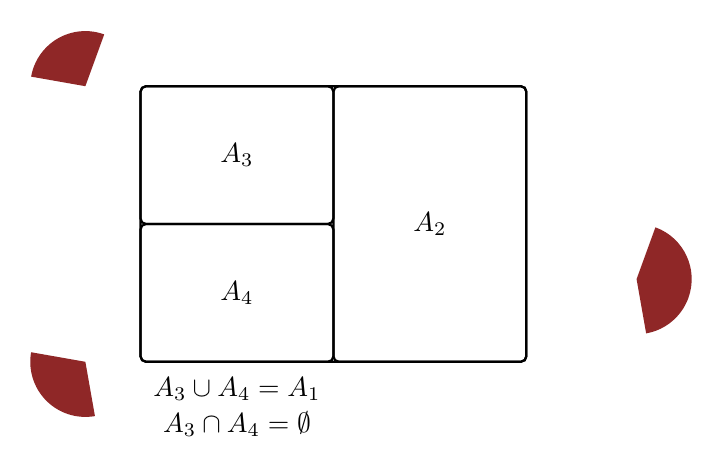
\begin{tikzpicture}[scale=0.35, thick]
  \draw [rounded corners=2pt, color=black] (4, 0) rectangle +(14, 10);
  \node at (7.5, -1) { $A_{3} \cup A_{4} = A_{1}$ };
  \node at (7.5, -2.25) { $A_{3} \cap A_{4} = \emptyset$ };

  \draw [rounded corners=2pt, color=black] (4, 5) rectangle +(7, 5) node[midway] { $A_{3}$ }; 
  \draw [rounded corners=2pt, color=black] (4, 0) rectangle +(7, 5) node[midway] { $A_{4}$ };
  
  \draw [rounded corners=2pt, color=black] (11, 0) rectangle +(7, 10) node[midway] { $A_{2}$ };
  
  \fill[color=dark] (2, 10) -- ({2 + 2 * sin(20)}, {10 + 2 * cos(20)}) arc (70:170:2) -- (2, 10);
  
  \fill[color=dark] (2, 0) -- ({2 - 2 * cos(10)}, {0 + 2 * sin(10)}) arc (170:280:2) -- (2, 0);  
  
  \fill[color=dark] (22, 3) -- ({22 + 2 * sin(20)}, {3 + 2 * cos(20)}) arc (70:-80:2) -- (22, 3);
\end{tikzpicture}

\end{document}  